\documentclass[10pt]{article}
%%%%%%%%%%%%%%% Define following before importing preamble
\def\Type{LessonCaelan}
\newcommand\TypeNum{Lesson 4}
\newcommand\TypeTitle{Limits at Infinity \\Notes To Instructor}
\newcommand\Semester{Fall 2021} %Not Used 
\newcommand\Course{MATH 1190 \& 1210}
\newcommand\Targets{ {\bf\color{RoyalBlue}L2}, {\bf\color{RoyalBlue}L2} }

%%%%%%%%%%%%%%%Preamble must come after above%%%%%%%
\usepackage{preambleDJ}



%%%%%%%%%%%% BEGIN DOCUMENT %%%%%%%%%%%%%%%
%%%%%%%%%%%% BEGIN DOCUMENT %%%%%%%%%%%%%%%
%%%%%%%%%%%% BEGIN DOCUMENT %%%%%%%%%%%%%%%
%%%%%%%%%%%% BEGIN DOCUMENT %%%%%%%%%%%%%%%
%%%%%%%%%%%% BEGIN DOCUMENT %%%%%%%%%%%%%%%

\begin{document}

\pagestyle{otherpages}
\thispagestyle{firstpage}
\vs{.75}
\lt  
\enumC{
\item[\target{L2}:] Continuity
\itemC{
    \item Identify the form of a limit. 
    \item Identify the method to use to evaluate a limit based on its form. 
    \item Evaluate a limit based on its form. 
}
}

~\\
\lg Students will be able to...
\enum{
\item Recognize  form $\dfrac{c}{\infty}$ occurs when dividing by larger and larger numbers and result gets smaller and smaller towards $0$. 
\item Recognize  form $\dfrac{\infty}{c}$ occurs when multiplying by larger and larger numbers and result gets bigger and bigger towards $\pm \infty$.  
\item Recognize form $\dfrac{\infty}{\infty}$ and how dominance hierarchy determines limit:  exp grows faster than polynomial grows faster than log functions.
\item Recognize form $\dfrac{\infty}{\infty}$ and how dominance hierarchy that leads to similarly growing terms (e.g. polynomial over polynomial) will require some algebra to find limit to $0$, $\infty$ or a constant value.  
\item  Recognize  form $\dfrac{c}{0}$ occurs when dividing by smaller and smaller numbers and result gets bigger and bigger towards $\pm \infty$. 
}

\feed. Feedback below is from F24. We're updating pre-class activity for S25, so {\em please check feedback from students before going to class.}
\itemC{
\item Many students found pre-class helpful and could see function behavior and how this led to limit conclusions.
\item Some commented that comparison between exponential, logarithmic and polynomial functions was helpful.
\item Some students were unclear about how to compute limits without calculator.
\item Some students were not as familiar with log functions. Other were less confident about exponential and polynomial functions in general.
\item Some found the epidemiology example confusing. 
}

 \hand
 \itemI{
 \item {\bf Warmup Exercise} is intended to help students connect limits towards infinity with graphs of functions and asymptotes (or not).
 \item Mini-lecture is a reminder of how Exponential, power, and log functions behave as $x$ approaches infinity.
 \item {\bf Limit Form 1 $\dfrac{c}{\infty}$} has three parts:  
 \enum{
 \item Poll is reminder (from pre-class work) on how functions of form $\dfrac{c}{\infty}$ behaves.
 \item Example 1 provides three examples instructor can work through.
 \item Exercise A has 3 examples students should work through. 
 }
 {\em Note 1}: It might be the case that students won't need instructor examples and can work through both instructor and student examples. In this case, we want to make sure all students have good summary of correct answers.\\
 {\em Note 2}: We're expecting much less algebraic work to compute limits compared to, say, Math 1310.  But we do want students to acknowledge the form they are seeing as part of their solution process. See solutions embedded below.
 \item {\bf Limit Form 2 $\dfrac{\infty}{c}$} has three parts.
 \enum{
 \item   Poll is reminder (from pre-class work) on how functions of form $\dfrac{\infty}{c}$ behaves.
 \item Example 2 provides three examples instructor can work through.
 \item Exercise B  t has 3 examples students should work through. Note: It might be the case that students won't need instructor examples and can work through both instructor and student examples. In this case, we want to make sure all students have good summary of correct answers.
 }
 {\em Note 3}: Again, students might be able to work most/all of Example and Exercise problems. Please require students articulate what form of a limit that are seeing that leads them to appropriate conclusion.
 \item {\bf Limit Form $\dfrac{\infty}{\infty}$}.  You will want to spend more time on this Limit Form and the one that follows as students will find this harder.  We again start with a Poll.  This is followed by a Mini-lecture where students are reminded of relative growth rates culminating in the Key Idea: Limits will be determined by dominant (i.e. fastest growing) term in numerator divided by same in denominator. \\\\
 Instructors will want to be clear about thinking as they work through Example 3. Exercise C will be great practice for students. This section concludes with a Summary of what students have seen in Example 3/Exercise C.
 \item {\bf Limit Form 4 $\dfrac{c}{0}$} It will be tight to finish this last Form and you may need to start the next class here. We again start with a Poll and a Mini-lecture. Example 4 and Exercise D both have problems that require checking two-sided limits.  
 }

\core Example 1/Exercise A, Example 2/Exercise B, Example 3/Exercise C and Example 4/Exercise D.

\newpage
\hrulefill ~\\
\textbf{Intended Learning Outcomes}
After this lesson, you will be able to 

\begin{itemize}
    \item Identify the form of a limit. (\target{L2})
    \item Identify the method to use to evaluate a limit based on its form. (\target{L2})
    \item Evaluate a limit based on its form. (\target{L2})
\end{itemize}

\vspace{-0.5cm}

\hrulefill
~\\
{\bf\color{blue}Warm-up Exercise 1.} Four graphs are given below.\\

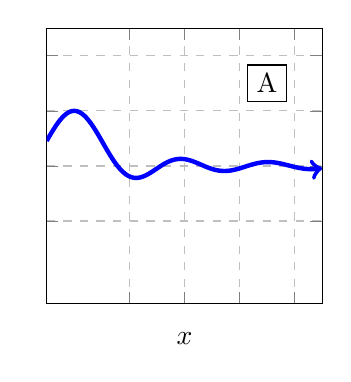
\begin{tikzpicture}[scale=1]
          \begin{axis}[
        %    axis y line = left,
        %    axis x line = bottom,
            xlabel={$x$},
            xtick       = {1,2,3,4},
            xticklabels = {},
            ytick       = {1,2,3,4},
            yticklabels = {},
            samples     = 160,
            domain      = -1:4.5,
            restrict y to domain=-1:4.5,
            xmin = -0.5, xmax = 4.5,
            ymin = -0.5, ymax = 4.5,
            grid=both, grid style=dashed,
            width=2in, height=2in
          ]
          % pieces 1 and 2
          \addplot[domain=-0.5:4.5, blue, ultra thick, ->] {2+sin(4*deg(x))/4/x};
          \node at (3.5,3.5) {\fbox{A}};
        \end{axis}
    \end{tikzpicture}
%
\hfill
%
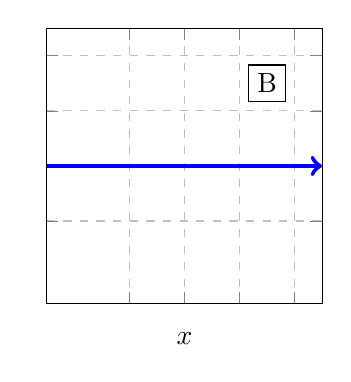
\begin{tikzpicture}[scale=1]
          \begin{axis}[
        %    axis y line = left,
        %    axis x line = bottom,
            xlabel={$x$},
            xtick       = {1,2,3,4},
            xticklabels = {},
            ytick       = {1,2,3,4},
            yticklabels = {},
            samples     = 160,
            domain      = -1:4.5,
            restrict y to domain=-1:4.5,
            xmin = -0.5, xmax = 4.5,
            ymin = -0.5, ymax = 4.5,
            grid=both, grid style=dashed,
            width=2in, height=2in
          ]
          % pieces 1 and 2
          \addplot[domain=-0.5:4.5, blue, ultra thick, ->] {2};
          \node at (3.5,3.5) {\fbox{B}};
        \end{axis}
    \end{tikzpicture}
%
\hfill
%
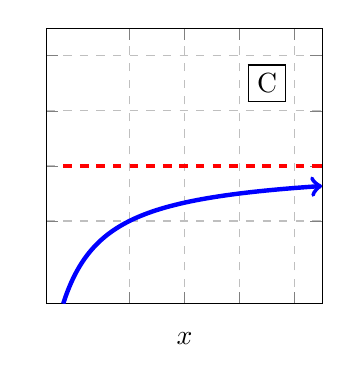
\begin{tikzpicture}[scale=1]
          \begin{axis}[
        %    axis y line = left,
        %    axis x line = bottom,
            xlabel={$x$},
            xtick       = {1,2,3,4},
            xticklabels = {},
            ytick       = {1,2,3,4},
            yticklabels = {},
            samples     = 160,
            domain      = -1:4.5,
            restrict y to domain=-1:4.5,
            xmin = -0.5, xmax = 4.5,
            ymin = -0.5, ymax = 4.5,
            grid=both, grid style=dashed,
            width=2in, height=2in
          ]
          % pieces 1 and 2
          \addplot[domain=-0.2:4.5, blue, ultra thick, ->] {2-2/(x+1)};
          \addplot[dashed, domain=-0.2:4.5, red, ultra thick, -] {2};
          \node at (3.5,3.5) {\fbox{C}};
        \end{axis}
    \end{tikzpicture}
%
\hfill
%
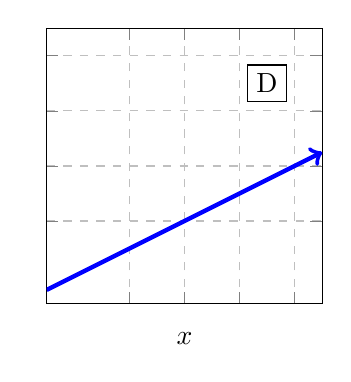
\begin{tikzpicture}[scale=1]
          \begin{axis}[
        %    axis y line = left,
        %    axis x line = bottom,
            xlabel={$x$},
            xtick       = {1,2,3,4},
            xticklabels = {},
            ytick       = {1,2,3,4},
            yticklabels = {},
            samples     = 160,
            domain      = -1:4.5,
            restrict y to domain=-1:4.5,
            xmin = -0.5, xmax = 4.5,
            ymin = -0.5, ymax = 4.5,
            grid=both, grid style=dashed,
            width=2in, height=2in
          ]
          % pieces 1 and 2
          \addplot[domain=-0.5:4.5, blue, ultra thick, ->] {0.5*x};
          \node at (3.5,3.5) {\fbox{D}};
        \end{axis}
    \end{tikzpicture}

For each statement below, decide which of the graphs appears to satisfy the statement. Specify all applicable answers.\\\nti{
Students will need to assume whether or not graph C has an  asymptote at $y=2$. For the purposes of this exercise, we assume it does. }
\begin{enumerate}
\item[(a)] $\displaystyle\lim_{x\to\infty}f(x)=2$ \dotfill \unline{1.5}{\blue{A, B, C}}{.25}\\
\item[(b)] $\displaystyle\lim_{x\to\infty}f(x)$ exists \dotfill \unline{1.5}{\blue{A, B, C}}{.25}\\
\item[(c)] $\displaystyle\lim_{x\to\infty}f(x)$ DNE\dotfill  \unline{1.5}{\blue{D.  Graph keeps increasing to $\infty$.}}{.25}\\
\end{enumerate}

\mpageT{.75}{.25}[\hs{.1}]{
\minil \mod {\it Functions with Infinite Limits at Infinity}
%{\em Exponentials \hfill Power Functions \hfill Logarithms}
\mpageTth{.32}{.33}{.32}{\centering
{\em Exponentials}\\
\blue{
Examples: $e^x$, $2^x$, $7^x$. Exponentials are all of form $a^x$: 
$$a^x\rightarrow \infty$$ when $a>1$.
}
}{\centering
{\em Power Functions }\\
\blue{
Examples: $x^2$, $x^{1/2}$, $x^7$, $x^{1/3}$. Power functions of form $x^n$.
$$x^n\rightarrow \infty$$ when $n>0$.
}
}{\centering
{\em Logarithms}
\blue{
Examples: $\ln(x)$, $\log_{10}(x)$, $\log_2(x)$.
Logarithms of form $\log_a(x)$
$$\log_a(x)\rightarrow \infty$$ when $a>1$.
}
}
}{
    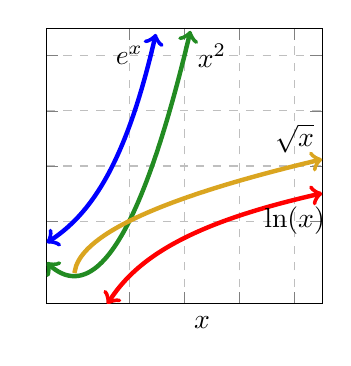
\begin{tikzpicture}[scale=1]
          \begin{axis}[
        %    axis y line = left,
        %    axis x line = bottom,
            xlabel={$x$},
            xtick       = {1,2,3,4},
            xticklabels = {},
            ytick       = {1,2,3,4},
            yticklabels = {},
            xlabel style={anchor=west},
            ylabel style={anchor=south},
            samples     = 160,
            domain      = -1:4.5,
            restrict y to domain=-1:4.5,
            xmin = -0.5, xmax = 4.5,
            ymin = -0.5, ymax = 4.5,
            grid=both, grid style=dashed,
            width=2in, height=2in
          ]
          % pieces 1 and 2
          \addplot[domain=-0.5:4.5, blue, ultra thick, <->] {e^x};
          \node at (2.5,4) {$x^2$};
          \addplot[domain=-0.5:4.5, ForestGreen, ultra thick, <->] {x^2};
          \node at (1,4) {$e^x$};
          \addplot[domain=-0.5:4.5, Goldenrod, ultra thick, ->] {x^(1/2)};
          \node at (4,2.5) {$\sqrt{x}$};
          \addplot[domain=0.6:4.5, red, ultra thick, <->] {ln(x)};
          \node at (4,1) {$\ln(x)$};
        \end{axis}
    \end{tikzpicture}
}
\\
\newpage
\lform   \blue{  \bf$\dfrac{c}{\infty}$} 


\exercise{\target{L2}} Use your knowledge of numbers and fractions to select an appropriate answer choice for the question below. If you aren't sure how to answer, then try to come up with some fractions in which the given situations occur to help you to form a guess.\\

When the {\it denominator} of a fraction grows ever larger without bound - all other things held constant - the value of the fraction...\\
\mpageT{.5}{.5}{
    \begin{enumerate}
    \item[A.] \blue{approaches $0$. See work in pre-class activity.}
    \item[B.] becomes larger.
    \item[C.] becomes larger without bound.
    \item[D.] could become larger, approach $0$, or anything in between based on the given information.
    \end{enumerate}
    }{
   \nti{  This problem is a good opportunity to use PollEverywhere.\\\\ Here's one way to illustrate the idea behind Form $\dfrac{c}{\infty}$.
$$
%\definecolor{Gray}{gray}{0.7}
%\newcolumntype{g}{>{\columncolor{Gray}}c}
\begin{array}{c |c|c|c|c}
 x&1&10&100&1000  \\ \hline
3/x&3&0.3&0.03&0.003
\end{array}
$$
}
}
    

%%%%%%%%%
\newpage%
%%%%%%%%%

\example{\color{RoyalBlue}L2} Find the following limits using forms: \\
\mpageTth{.33}{.35}{.33}{
$\displaystyle\lim_{x\to\infty} \frac{1}{x^5}=$ \unline{.5}{\blue{0}}{.25}\\
\blue{
Since $x^5 \rightarrow \infty$ we have\\
Form $\dfrac{1}{\infty}$. We know this \\approaches $0$.
}
}{
$\displaystyle\lim_{x\to\infty} \frac{10}{\log_4(x)+\sqrt{x-4}}=$ \unline{.5}{\blue{0}}{.25}\\
\blue{
Since $\log_4(x)\to \infty$ and \\
$(x-4)^{1/2}\to \infty$,  denominator \\
approaches $\infty$. \\Form is $\dfrac{10}{\infty}$ which \\approaches $0$.
}
}{
$\displaystyle\lim_{x\to\infty} 6e^{-x}=$ \unline{.5}{\blue{0}}{.25}\\
\blue{
$6e^{-x}=\dfrac{6}{e^x}$. Since $e^x\to \infty$, Form is $\dfrac{6}{\infty}$ which approaches $0$.
}
}
\vfill

\exercise{\color{RoyalBlue}L2} Find the following limits using forms. (Practice showing your work, even if you know the answer!) \\
\mpageTth{.33}{.33}{.33}{
$\displaystyle\lim_{x\to\infty} 5x^{-3}=$ \unline{.5}{\blue{0}}{.25}\\
\blue{
$5x^{-3}=\dfrac{5}{x^3}$. $x^3\to\infty$ \\Form is $\dfrac{5}{\infty}$ which \\approaches $0$.
}
}{
$\displaystyle\lim_{x\to\infty} -\frac{1}{e^x+x^{1000}}=$ \unline{.5}{\blue{0}}{.25}\\
\blue{
Both $e^x\to \infty$ and \\$x^{1000}\to \infty$ so $e^x+x^{1000}\to \infty$. \\Form is $\dfrac{1}{\infty}$ which \\approaches $0$.
}
}{
$\displaystyle\lim_{x\to\infty} \frac{e^{-x}}{x^2} =$ \unline{.5}{\blue{0}}{.25}\\
\blue{
$\dfrac{e^{-x}}{x^2}=\dfrac{1}{e^{x}\cdot x^2}$.  Both $e^x\to\infty$ and $x^2\to\infty$. Thus $e^x \cdot x^2\to \infty$ and Form is $\dfrac{1}{\infty}$ which approaches $0$.
}
}

\vfill


\lform  \blue{\bf $\dfrac{\infty}{c}$ }


\exercise{\target{L2}} Use your knowledge of numbers and fractions to select an appropriate answer choice for the question below. If you aren't sure how to answer, then try to come up with some fractions in which the given situations occur to help you to form a guess.\\

When the {\it numerator} of a fraction grows ever larger without bound - all other things held constant - the value of the fraction...\\
\mpageT{.5}{.5}{
    \begin{enumerate}
    \item[A.] approaches $0$.
    \item[B.] becomes larger.
    \item[C.] \blue{becomes larger without bound. See pre-class work. }
    \item[D.] could become larger, approach $0$, or anything in between based on the given information.
    \end{enumerate}
}{
\nti{ This problem is a good opportunity to use PollEverywhere.\\
 Here's one way to illustrate the idea behind Form $\dfrac{\infty}{c}$.
$$
%\definecolor{Gray}{gray}{0.7}
%\newcolumntype{g}{>{\columncolor{Gray}}c}
\begin{array}{c |c|c|c|c}
 x&1&10&100&1000  \\ \hline
x/3&1/3&10/3&100/3&1000/3
\end{array}
$$
}
}\vs{.1}\\ 
\example{\color{RoyalBlue}L2} Find the following limits using forms:\vs{-.2}\\
\mpageTth{.33}{.33}{.33}{
$\displaystyle\lim_{x\to\infty} \frac{e^x+1}{2}=$ \unline{.5}{\blue{$\infty$} }{.25}\\
\blue{
$e^x+1\to \infty$ so Form is $\dfrac{\infty}{2}$ \\which approaches $\infty$.
}
}{
$\displaystyle\lim_{x\to\infty} \frac{-2x^2}{3\sqrt[4]{x}}=$ \unline{.5}{\blue{-$\infty$}}{.25}\\
\blue{
$\dfrac{-2x^2}{3\sqrt[4]{x}}=\dfrac{-2x^2}{3x^{1/4}}\\
=\dfrac{-2x^2\cdot x^{-1/4}}{3}=\dfrac{-2x^{2-1/4}}{3}\\
=\dfrac{-2x^{7/4}}{3}$.  $-2x^{7/4}\to -\infty$ so Form is $\dfrac{-\infty}{3}$ which approaches $-\infty$. 
}
}{
$\displaystyle\lim_{x\to\infty} \frac{1-\ln(x)}{-3}=$ \unline{.5}{\blue{$\infty$}}{.25} \\
\blue{
$\ln(x)\to\infty$ so $1-\ln(x)\to -\infty$.  Form is $\dfrac{-\infty}{-3}$ which approaches $+\infty$.
}
}
\exercise{\color{RoyalBlue}L2} Find the following limits using forms. (Practice showing your work, even if you know the answer!)\vs{-.2}\\
\mpageTth{.33}{.33}{.33}{
$\displaystyle\lim_{x\to\infty} -\frac{\sqrt{x}}{5}=$ \unline{.5}{ \blue{-$\infty$} }{.25}\\
\blue{
$\sqrt{x}\to \infty$ so Form is $-\dfrac{\infty}{5}$ \\
which approaches $-\infty$.
}
}{
$\displaystyle\lim_{x\to\infty} \frac{x^5}{2x}=$ \unline{.5}{ \blue{$\infty$} }{.25}\\
\blue{
$\dfrac{x^5}{2x}=\dfrac{x^4}{2}$. Since $x^4\to\infty$ \\
Form is $\dfrac{\infty}{2}$ which \\approaches $\infty$.
}
}{ 
$\displaystyle\lim_{x\to\infty} \frac{1}{2e^{-x}}=$ \unline{.5}{ \blue{$\infty$} }{.25}\\
\blue{
$\dfrac{1}{2e^{-x}}=\dfrac{e^x}{2}$.  Since $e^x\to\infty$ Form is $\dfrac{\infty}{2}$ which approaches $\infty$.
}
}



%%%%%%%%%
\newpage%
%%%%%%%%%
%$\left({\it \text{\bf \blue{Form} }\dfrac{\infty}{\infty}}\right)$
\lform  \blue{\bf $\dfrac{\infty}{\infty}$}


\exercise{\target{L2}}  Use your knowledge of numbers and fractions to select an appropriate answer choice for the question below. If you aren't sure how to answer, then try to come up with some fractions in which the given situations occur to help you to form a guess.\\

When both the {\it numerator and denominator} grow ever larger without bound, the value of the fraction...\\
\mpageT{.5}{.5}{
    \begin{enumerate}
    \item[A.] approaches $0$.
    \item[B.] becomes larger.
    \item[C.] becomes larger without bound.
    \item[D.] \blue{could become larger, approach $0$, or anything in between based on the given information.}
    \end{enumerate}
}{
\nti{This question is a good opportunity to use PollEverywhere}
}\\
%%%

\mpageT{.75}{.25}[\hs{.1}]{
{\bf\color{blue}Mini-lecture. }\mod {\it Functions with Infinite Limits at Infinity}
%{\em Exponentials \hfill Power Functions \hfill Logarithms}
\mpageTth{.32}{.33}{.32}[\hs{.1}][\hs{.1}]{{\centering
{\em Exponentials}}\\
\blue{
Exponential functions such as $e^x$ grow much faster than other functions we will see. The general form is $a^x$ where $a>1$.
}
}{{\centering
{\em Power Functions }}\\
\blue{
Power functions such as $x^2$ or $x^{1/2}$ grow much faster than logarithmic functions and slower than exponential functions. The general form is $x^n$ where $n>0$. {\em Within power functions}, larger exponents mean faster growth.
}
}{{\centering
{\em Logarithms}}\\
\blue{
Slowest growing.
}
}
}{
    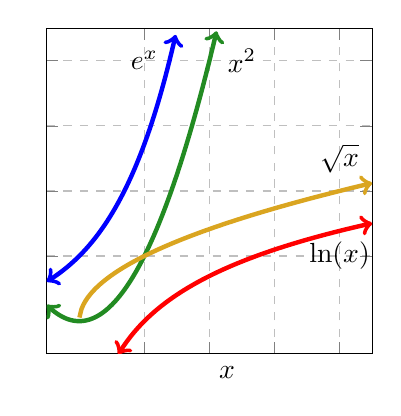
\begin{tikzpicture}[scale=1]
          \begin{axis}[
        %    axis y line = left,
        %    axis x line = bottom,
            xlabel={$x$},
            xtick       = {1,2,3,4},
            xticklabels = {},
            xlabel style={anchor=west},
            ytick       = {1,2,3,4},
            yticklabels = {},
            ylabel style={anchor=south},
            samples     = 160,
            domain      = -1:4.5,
            restrict y to domain=-1:4.5,
            xmin = -0.5, xmax = 4.5,
            ymin = -0.5, ymax = 4.5,
            grid=both, grid style=dashed,
            width=2.25in, height=2.25in
          ]
          % pieces 1 and 2
          \addplot[domain=-0.5:4.5, blue, ultra thick, <->] {e^x};
          \node at (2.5,4) {$x^2$};
          \addplot[domain=-0.5:4.5, ForestGreen, ultra thick, <->] {x^2};
          \node at (1,4) {$e^x$};
          \addplot[domain=-0.5:4.5, Goldenrod, ultra thick, ->] {x^(1/2)};
          \node at (4,2.5) {$\sqrt{x}$};
          \addplot[domain=0.6:4.5, red, ultra thick, <->] {ln(x)};
          \node at (4,1) {$\ln(x)$};
        \end{axis}
    \end{tikzpicture}
}
{\em Key Idea for Form $\dfrac{\infty}{\infty}$}\\
\blue{We're going to choose the Dominant Term (i.e. the fastest growing) in both the numerator and denominator to create a new fraction. This new fraction will have the same limit as our original.} \\\\
\example{\color{RoyalBlue}L2} Find the following limits using forms:\\
\mpageTth{.33}{.33}{.36}[\hs{.15}][\hs{.15}]{
$\displaystyle\lim_{x\to\infty} \frac{\log_2(x)}{x^3+4x-1}=$ \unline{.5}{ \blue{$0$} }{.25}\\
\blue{
\itemC{
\item Dominant term in numerator: $\log_2(x)$\\
\item Dominant term in denominator: $x^3$.\\
\item $\ds \lim_{x\to\infty} \frac{\log_2(x)}{x^3+4x-1} $\\
$\ds \qquad \qquad \sim \lim_{x\to\infty} \frac{\log_2(x)}{x^3}$\\
\item Form is $\dfrac{\infty}{\infty}$ with\\ 
$\dfrac{slower}{much\,\, faster}\to 0$. \\
\item Thus $\ds \lim_{x\to\infty} \frac{\log_2(x)}{x^3}=0$\\
$\ds \Rightarrow \lim_{x\to\infty} \frac{\log_2(x)}{x^3+4x-1}=0$
}
}
}{
$\displaystyle\lim_{x\to\infty} \frac{4^x+\ln(x)}{1-\sqrt[3]{x}}=$ \unline{.5}{ \blue{$-\infty$} }{.25} \\
\blue{
\itemC{
\item Dominant term in numerator: $4^x$\\
\item Dominant term in denominator: $-\sqrt[3]{x}=-x^{1/3}$.\\
\item $\ds \lim_{x\to\infty} \frac{4^x+\ln(x)}{1-\sqrt[3]{x}} \sim \lim_{x\to\infty} \frac{4^x}{-x^{1/3}}$\\
\item Form is $\dfrac{\infty}{-\infty}$ with\\ 
$\dfrac{much\,\,faster}{-slower}\to -\infty$.\\
\item Thus $\ds \lim_{x\to\infty} \frac{4^x}{-x^{1/3}}=-\infty$\\
$\ds \Rightarrow \lim_{x\to\infty} \frac{4^x+\ln(x)}{1-\sqrt[3]{x}} =-\infty$
}
}
}{
$\displaystyle\lim_{x\to\infty} \frac{\log_2(x)-\sqrt{x}}{2\sqrt{x+5}-4}=$ \unline{.5}{ \blue{$-\dfrac{1}{2}$} }{.25}\\
\blue{
\itemC{
\item Dominant term in numerator: $-\sqrt{x}$
\item Dominant term in denominator: $2\sqrt{x}$. (The ``$+5$" portion of $2\sqrt{x+5}$ is not growing).
\item $\ds \lim_{x\to\infty} \frac{\log_2(x)-\sqrt{x}}{2\sqrt{x+5}-4} \sim \lim_{x\to\infty} \frac{-\sqrt{x}}{2\sqrt{x}}$\\
$\ds =\lim_{x\to \infty} \frac{-1}{2}=-\frac{1}{2}$
\item Thus $\ds \lim_{x\to\infty} \frac{-\sqrt{x}}{2\sqrt{x}}=-\frac{1}{2}$\\
$\ds \Rightarrow \lim_{x\to\infty} \frac{\log_2(x)-\sqrt{x}}{2\sqrt{x+5}-4}=-\frac{1}{2}$
}
}
}


\newpage
\exercise{\color{RoyalBlue}L2} Find the following limits using forms. (Practice showing your work, even if you  know the answer!)\\
\mpageTth{.33}{.35}{.36}[\hs{.15}][\hs{.15}]{
$\displaystyle\lim_{x\to\infty} \frac{7^x-x}{x^7}=$ \unline{.5}{ \blue{$\infty$}}{.25}\\
\blue{
\itemC{
\item Dominant term in numerator: $7^x$
\item Dominant term in denominator: $x^7$.
\item $\ds \lim_{x\to\infty} \frac{7^x-x}{x^7}\sim \lim_{x\to\infty} \frac{7^x}{x^7}$
\item Form is $\dfrac{\infty}{\infty}$ with\\ 
$\dfrac{much \,\,faster}{slower}\to \infty$. 
\item Thus $\ds \lim_{x\to\infty} \frac{7^x}{x^7}=\infty$\\
$\ds \Rightarrow  \lim_{x\to\infty} \frac{7^x-x}{x^7}=\infty$
}
}
}{
$\displaystyle\lim_{x\to\infty} \frac{\sqrt{x+1}}{4-x-\ln(x)}=$ \unline{.5}{ \blue{$0$}}{.25}\\
\blue{
\itemC{
\item Dominant term in numerator: $\sqrt{x}$. (The ``$+1$" is not growing)
\item Dominant term in denominator: $-x$.
\item $\ds \lim_{x\to\infty} \frac{\sqrt{x+1}}{4-x-\ln(x)}\sim \lim_{x\to\infty} \frac{\sqrt{x}}{-x}$
\item This simplifies further:\\
$$\ds \lim_{x\to\infty} \frac{x^{1/2}}{-x}=\frac{1}{-x^{1/2}}$$
\item Form $\dfrac{1}{-\infty}$ which approaches $0$.
\item $\ds \lim_{x\to\infty} \frac{\sqrt{x}}{-x}=0$\\
$\ds \Rightarrow \lim_{x\to\infty} \frac{\sqrt{x+1}}{4-x-\ln(x)}=0$
}
}
}{
$\displaystyle\lim_{x\to\infty} \frac{\sqrt{x^2+1}}{4-3x-\ln(x)}=$ \unline{.5}{ \blue{$\ds -\frac{1}{3}$} }{.25}\\
\blue{
\itemC{
\item Dominant term in numerator: $\sqrt{x^2}$. (The ``$+1$" is not growing)
\item Dominant term in denominator: $-3x$.
\item $\ds \lim_{x\to\infty} \frac{\sqrt{x^2+1}}{4-3x-\ln(x)} \sim \lim_{x\to\infty} \frac{\sqrt{x^2}}{-3x}$
\item This simplifies:\\
$$\lim_{x\to\infty} \frac{\sqrt{x^2}}{-3x}=\lim_{x\to\infty} \frac{x}{-3x}=\lim_{x\to\infty}\frac{1}{-3}=-\frac{1}{3}$$
($\sqrt{x^2}=x$ for $x>0$)
\item $\ds  \lim_{x\to\infty} \frac{\sqrt{x^2}}{-3x}=-\frac{1}{3}$\\
$\ds \Rightarrow \lim_{x\to\infty} \frac{\sqrt{x^2+1}}{4-3x-\ln(x)}=-\frac{1}{3}$
}
}
}

\mpageTth{.33}{.33}{.36}[\hs{.15}][\hs{.15}]{
$\displaystyle\lim_{x\to\infty} \frac{1000-x^{1000}}{x^e-e^x}=$ \unline{.5}{ \blue{$0$}}{.25}\\
\blue{
\itemC{
\item Dominant term in numerator: $-x^{1000}$. 
\item Dominant term in denominator: $-e^x$.
\item $\ds \lim_{x\to\infty} \frac{1000-x^{1000}}{x^e-e^x} \\$
$\ds \qquad \sim \lim_{x\to\infty} \frac{-x^{1000}}{-e^x}$
\item \item Form is $\dfrac{\infty}{\infty}$ with\\ 
$\dfrac{slower}{much \,\,faster}\to 0$. 
\item $\ds \lim_{x\to\infty} \frac{-x^{1000}}{-e^x}=0$\\
$\ds \Rightarrow \lim_{x\to\infty} \frac{1000-x^{1000}}{x^e-e^x}=0$
}
}
}{
$\displaystyle\lim_{x\to\infty} \frac{5e^{2x}+3e^x+1}{e^{2x}-5e^x+6}=$ \unline{.5}{ \blue{$5$}}{.25} \\
\blue{
\itemC{
\item Dominant term in numerator: $5e^{2x}$. 
\item Dominant term in denominator: $e^{2x}$.
\item $\ds \lim_{x\to\infty} \frac{5e^{2x}+3e^x+1}{e^{2x}-5e^x+6} $\\
$\ds \qquad \qquad \sim \lim_{x\to\infty} \frac{5e^{2x}}{e^{2x}}$
\item This simplifies further:
$$\lim_{x\to\infty} \frac{5e^{2x}}{e^{2x}}=\lim_{x\to\infty} \frac{5}{1}=5$$
\item $\ds \lim_{x\to\infty} \frac{5e^{2x}}{e^{2x}}=5$\\
$\ds \Rightarrow \lim_{x\to\infty} \frac{5e^{2x}+3e^x+1}{e^{2x}-5e^x+6}=5$
}
}
}{
%$\displaystyle\lim_{x\to\infty} \frac{x^5 +3x+\ln(x)}{2x+3}=$ \unline{.5}{}{.25} \\
\blue{
%
}
}
\vs{.5}~\\
\blue{\bf Summary of Limit Form   $\dfrac{\infty}{\infty}$}
After choosing dominant terms in numerator and denominator....
\itemI{
\item $\ds \frac{\text{much faster}}{\text{slower}}\to$ \blue{$\ds \pm \infty$}
\vs{.75}
\item $\ds \frac{\text{slower}}{\text{much faster}}\to$  \blue{$\ds \pm \infty$}
\vs{.75}
\item $\ds \frac{\text{about the same}}{\text{about the same}}\to$  \blue{Do some algebra to see if limit simplifies to another form.}
}

%%%%%%%%%

%%%%%%%%%
\newpage
%$\left({\it \text{\bf \blue{Form} }\dfrac{c}{0}}\right)$
\lform $\blue{\bf \dfrac{c}{0}}$



\exercise{\target{L2}}  Use your knowledge of numbers and fractions to select an appropriate answer choice for the question below. If you aren't sure how to answer, then try to come up with some fractions in which the given situations occur to help you to form a guess.\\

When the {\it denominator} of a fraction grows ever smaller - approaching $0$ - with all other things held constant, the value of the fraction...\\
\mpageT{.5}{.5}{
    \begin{enumerate}
    \item[A.] approaches $0$.
    \item[B.] becomes larger.
    \item[C.] \blue{becomes larger without bound.}
    \item[D.] could become larger, approach $0$, or anything in between based on the given information.
    \end{enumerate}
}{
\nti{  This is a good question to use PollEverywhere.\\ Here's one way to illustrate the idea behind Form $\dfrac{c}{0}$.
$$
%\definecolor{Gray}{gray}{0.7}
%\newcolumntype{g}{>{\columncolor{Gray}}c}
\begin{array}{c |c|c|c|c}
 x&1&1/10&1/100&1/1000  \\ \hline
3/x&3&30&300&3000
\end{array}
$$
}
}
\vs{.1}\\
\minil \mod What can be said about a limit if we know its form resembles $\dfrac{c}{0}$? Specify the various cases as well as what you can conclude in each of those cases.\\
\mpageT{.5}{.5}[\hs{.1}]{
\nti{
In all cases of Form $\dfrac{c}{0}$, the limit DNE.  But {\em how} we get to DNE is important.
}
}{
\begin{flushright}
\begin{tabular}{|>{\columncolor{lightgray}}c|c|c|}  \hline
\rowcolor{lightgray}&\hs{1}&\hs{1}\\
\rowcolor{lightgray}$\ds \to\frac{c}{0}$&Num $\to (+)$&Num $\to (-)$\\ 
\rowcolor{lightgray}&& \\ \hline
&&\\
Denom $\to 0^+$ &\blue{Form: $\dfrac{+c}{0^+} \to +\infty$}& \blue{Form: $\dfrac{-c}{0^+} \to -\infty$} \\ 
&&\\
&& \\ \hline
&&\\
Denom $\to 0^-$& \blue{Form: $\dfrac{+c}{0^-}\to -\infty$}& \blue{Form: $\dfrac{-c}{0^-} \to +\infty$}\\
&&\\
&&\\ \hline
\end{tabular}
\end{flushright}
}
\vfill
\vfill

\newpage

\example{\color{RoyalBlue}L2} Find the following limits using forms:
	\enumA{
\mpageT{.5}{.5}[\hs{.1}]{
	\item $\displaystyle\lim_{x\to1^{-}} \frac{\sqrt{x}+1}{x-1}=$\unline{1}{ \blue{$-\infty$}}{.25}\\
	\blue{
	Since $x\to 1^-$, $x-1\to0^-$. Form is $\dfrac{2}{0^-}$ \\which approaches $-\infty$. \\That is, $\ds \lim_{x\to1^{-}} \frac{\sqrt{x}+1}{x-1}$
	}
	}{
	\item $\displaystyle\lim_{x\to3} \frac{x^2-2x}{3-x}=$\unline{1}{ \blue{DNE}}{.25}\\
	\blue{
		Since $x\to 3$ we must consider the two-sided limit.
		\itemI{
		\item $\ds \lim_{x\to3^-} \frac{x^2-2x}{3-x} \to \frac{3^2-2\cdot 3}{0^+}$\\
		 Form is $\dfrac{3}{0^+}\to \infty$.  Thus $\ds \lim_{x\to3^-} \frac{x^2-2x}{3-x}=\infty$
		 \item $\ds \lim_{x\to3^+} \frac{x^2-2x}{3-x} \to \frac{3^2-2\cdot 3}{0^-}$\\
		 Form is $\dfrac{3}{0^-}\to -\infty$.  Thus $\ds \lim_{x\to3^+} \frac{x^2-2x}{3-x}=-\infty$
		 \item Since $\ds \lim_{x\to3^-} \frac{x^2-2x}{3-x} = \infty \neq  \lim_{x\to3^+} \frac{x^2-2x}{3-x}$,\\ $\ds \lim_{x\to3} \frac{x^2-2x}{3-x}$ DNE.
		}
		}
	}
	\vs{.5}\\
\exercise{\color{RoyalBlue}L2} Find the following limits using forms:\\
\mpageT{.5}{.5}[\hs{.1}]{
	\item $\displaystyle\lim_{x\to 0^+}\frac{1+x}{x^2}=$\unline{1}{ \blue{$\infty$} }{.25}\\
	\blue{
	Since $x\to 0^+$, $1+x\to 1$ and $x^2\to 0^+$. \\
	Form is $\dfrac{1}{0^+}$ which approaches $\infty$. \\
	Thus $\displaystyle\lim_{x\to 0^+}\frac{1+x}{x^2}=\infty$.
	}
}{
\item $\displaystyle\lim_{x\to 5}\frac{1+x}{x^2-25}=$\unline{1}{ \blue{DNE}}{.25}\\
	\blue{
	We must consider two-sided limit.
	\itemI{
	\item $\ds \lim_{x\to 5^-}\frac{1+x}{x^2-25}$.  Since $x\to 5^-$, $1+x\to 6$ and $x^2-25\to 0^-$.  Form is $\dfrac{6}{0^-}$ approaches $-\infty$.  That is $\ds \lim_{x\to 5^-}\frac{1+x}{x^2-25}=-\infty$.
	\item $\ds \lim_{x\to 5^+}\frac{1+x}{x^2-25}$ Since $x\to 5^-$, $1+x\to 6$ and $x^2-25\to 0+$. Form is $\dfrac{6}{0^+}$ approaches $+\infty$.  That is $\ds \lim_{x\to 5^+}\frac{1+x}{x^2-25}=+\infty$.
	\item Since $\ds \lim_{x\to 5^-}\frac{1+x}{x^2-25} \neq  \lim_{x\to 5^+}\frac{1+x}{x^2-25}$, $\ds \lim_{x\to 5}\frac{1+x}{x^2-25} = DNE$
	}
	}
}
	}

%%%%%%%%%
\newpage%
%%%%%%%%%

{\bf\color{blue}Extra Practice 1.}\reversemarginpar\marginnote{\fbox{\bf\color{RoyalBlue}L2}} Find the following limits using either forms or continuity.\\
\enumA{
\mpageT{.5}{.5}{
\item $\displaystyle\lim_{x\to1^+} (1-x)^{-3} $ \\
\blue{
\itemI{
\item $\ds \lim_{x\to1^+} (1-x)^{-3}=\lim_{x\to1^+} (\frac{1}{1-x)^3} $. 
\item As $x\to1^+$, $(1-x)^3\to (0^-)^3=0^-$.  
\item Form is $\dfrac{1}{0^-}\to -\infty$. 
\item Thus $\displaystyle\lim_{x\to1^+} (1-x)^{-3}=-\infty$.
}
}
}{ 
\item $\displaystyle\lim_{x\to\infty} (1-x)^{-3}$\\
\blue{
\itemI{
\item As $x\to\infty$, $1-x\to -\infty$. 
\item Thus $\ds\lim_{x\to\infty} (1-x)^{-3}=\lim_{x\to\infty} \frac{1}{(1-x)^3}$ 
\item This is of Form $\dfrac{1}{-\infty}\to 0$
\item Thus$\displaystyle\lim_{x\to\infty} (1-x)^{-3}=0$
}
}
}

\mpageT{.5}{.5}{
\item $\displaystyle\lim_{x\to\infty} \frac{x^2-4x-\sqrt{x}}{1-\sqrt[3]{x^2-2x}}$  \\
\blue{
\itemI{
\item $\displaystyle\lim_{x\to\infty} \frac{x^2-4x-\sqrt{x}}{1-\sqrt[3]{x^2-2x}} \sim \lim_{x\to\infty} \frac{x^2}{-\sqrt[3]{x^2}} $
\item This simplifies further:\\
\al{
 \lim_{x\to\infty} \frac{x^2}{-\sqrt[3]{x^2}}&= \lim_{x\to\infty} \frac{x^2}{-x^{2/3}}\\
&=\lim_{x\to\infty} \frac{x^2\cdot x^{-2/3}}{-1}\\
&=\lim_{x\to\infty} \frac{x^{4/3}}{-1}
\intertext{This is Form $\dfrac{\infty}{-1}\to -\infty$. Thus }
 \lim_{x\to\infty} \frac{x^2}{-\sqrt[3]{x^2}}&= -\infty
}
}
}
}{ 
\item $\displaystyle\lim_{x\to4} \frac{x^2-4x-\sqrt{x}}{1-\sqrt[3]{x^2-2x}}$ \\
\blue{
\itemI{
\item Note that this problem differs from c) in that we're finding limit as $x\to 4$ instead of limit as $x\to\infty$. At $x=4$, each component of function is continuous.  In particular $x^2$, $-4x$, $\sqrt{x}$, $1$, and $-\sqrt[3]{x^2-2x}$ are all continuous when $x=4$.  
\item So we're going to use the fact about continuous functions: $$\lim_{x\to a}f(x)=f(a).$$
\item 
\al{
\lim_{x\to4} \frac{x^2-4x-\sqrt{x}}{1-\sqrt[3]{x^2-2x}}&= \frac{4^2-4\cdot 4-\sqrt{4}}{1-\sqrt[3]{4^2-2\cdot 4}}\\
&=\frac{16-16-2}{1-\sqrt[3]{8}}\\
&=\frac{-2}{-1}\\
&=2
}
\item {\em Caveat} In this problem,  we have a situation  $\ds f(x)=\frac{g(x)}{h(x)}$ where both $g(x)=x^2-4x-\sqrt{x}$ and $\ds h(x)=1-\sqrt[3]{x^2-2x}$ are both continuous at $x=4$.  We used the fact that dividing two continuous functions to get $\ds \frac{g(x)}{h(x)}$ results in another continuous function. This is true {\em except for the case when $h(x)=0$}.  For example, if we would have had $$\lim_{x\to4} \frac{x^2-4x-\sqrt{x}}{x-4}$$ both $\ds g(x)=x^2-4x-\sqrt{x}$ and $h(x)=x-4$ are continuous at $x=4$.  But, since $h(4)=0$, $\ds f(x)=\frac{g(x)}{h(x)}$ is {\em not} continuous at $x=4$. In this situation we would want to utilize fact $$\lim_{x\to4} \frac{x^2-4x-\sqrt{x}}{x-4}\to \frac{c}{0}$$ and proceed from there.
}
}
}
\newpage
\mpageT{.5}{.5}{
\item $\displaystyle\lim_{x\to\infty} \dfrac{\sqrt[3]{x^7+1}-x}{\ln(x)+x^2} $  \\
\blue{
\itemI{
\item $\displaystyle\lim_{x\to\infty} \dfrac{\sqrt[3]{x^7+1}-x}{\ln(x)+x^2} \sim \lim_{x\to\infty} \dfrac{\sqrt[3]{x^7}-x}{x^2} $
\item This simplifies further
\al{
\lim_{x\to\infty} \dfrac{\sqrt[3]{x^7}-x}{x^2} &=\lim_{x\to\infty} \dfrac{x^{7/3}}{x^2} \\
&=\lim_{x\to\infty} x^{7/3 -2}\\
&=\lim_{x\to\infty} x^{7/3 -6/3}\\
&=\lim_{x\to\infty} x^{1/3}\\
&=\infty
}
\item Thus $\displaystyle\lim_{x\to\infty} \dfrac{\sqrt[3]{x^7+1}-x}{\ln(x)+x^2} =\infty$.
}
}
}{
\item $\displaystyle\lim_{x\to\infty} \dfrac{\ln(x)+x^2}{\sqrt[3]{x^7+1}-x}$ \\
\blue{
\itemI{
\item $\displaystyle\lim_{x\to\infty} \dfrac{\ln(x)+x^2}{\sqrt[3]{x^7+1}-x} \sim \lim_{x\to\infty} \dfrac{x^2}{\sqrt[3]{x^7+1}}$
\item This simplifies further:
\al{
\lim_{x\to\infty} \dfrac{x^2}{\sqrt[3]{x^7}-x}&=\lim_{x\to\infty} \dfrac{x^2}{x^{7/3}} \\
&=\lim_{x\to\infty} \frac{1}{x^{7/3 -2}}\\
&=\lim_{x\to\infty} \frac{1}{x^{7/3 -6/3}}\\
&=\lim_{x\to\infty} \frac{1}{x^{1/3}}\\
\intertext{This is form $\dfrac{1}{\infty}$}
&=0
}
\item Thus $\displaystyle\lim_{x\to\infty} \dfrac{\ln(x)+x^2}{\sqrt[3]{x^7+1}-x}=0$
}
}
}

\mpageT{.5}{.5}{
\item $\displaystyle\lim_{x\to\infty} \frac{e^x+e^{-x}}{e^x-e^{-x}} $  \\
\blue{
\itemI{
\item $e^x$ grows while $e^{-x}$ decays (i.e. decreases) \\as $x\to \infty$. 
\item $\displaystyle\lim_{x\to\infty} \frac{e^x+e^{-x}}{e^x-e^{-x}} \sim \lim_{x\to\infty} \frac{e^x}{e^x} $
\item $\ds\lim_{x\to\infty} \frac{e^x}{e^x}=\lim_{x\to\infty} 1=1$
\item Thus $\displaystyle\lim_{x\to\infty} \frac{e^x+e^{-x}}{e^x-e^{-x}} =1$ 
}
}
\vs{1}
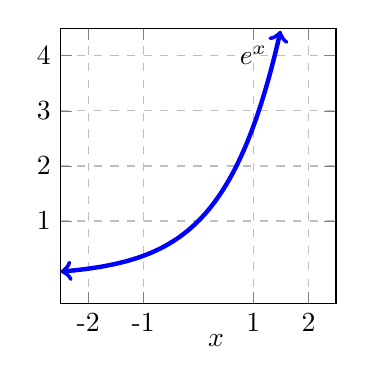
\begin{tikzpicture}[scale=1]
          \begin{axis}[
        %    axis y line = left,
        %    axis x line = bottom,
            xlabel={$x$},
            xtick       = {-2,-1,1,2,3,4},
            xticklabels = {-2,-1,1,2,3,4},
            xlabel style={anchor=west},
            ytick       = {1,2,3,4},
            yticklabels = {1,2,3,4},
            ylabel style={anchor=south},
            samples     = 160,
            domain      = -2:2.5,
            restrict y to domain=-.5:4.5,
            xmin = -2.5, xmax = 2.5,
            ymin = -0.5, ymax = 4.5,
            grid=both, grid style=dashed,
            width=2in, height=2in
          ]
          % pieces 1 and 2
          \addplot[domain=-2.5:2.5, blue, ultra thick, <->] {e^x};
            \node at (1,4) {$e^x$};
        \end{axis}
    \end{tikzpicture}
    \hs{-1.5}\captionof*{figure}{Graph for part (h)}
}{
 \item $\displaystyle\lim_{x\to0^-} \frac{e^x+e^{-x}}{e^x-e^{-x}} $ \\
\blue{
\itemI{
\item The difference between this problem and g) is limit is as $x\to 0^-$ here instead of $x\to \infty$.
\item Every component of $\ds \frac{e^x+e^{-x}}{e^x-e^{-x}} $ is continuous at $x=0$ 
\item As $x\to 0^-$, the numerator $e^x+e^{-x}\to 1+1=2$
\item {\em However} as $x\to 0^-$ in the denominator we have  \\
$\ds \lim_{x\to0^-} e^{x}-e^{-x}\to 1-1=0$ and thus $\ds \frac{e^x+e^{-x}}{e^x-e^{-x}} $ is {\em not } continuous at $x=0$.
\item But we note that the Form is $\displaystyle\lim_{x\to0^-} \frac{e^x+e^{-x}}{e^x-e^{-x}} \to \frac{2}{0}$
\item We need to further decide if From = $\dfrac{2}{0^-}$ or if Form =  $\dfrac{2}{0^+}$
\item $\ds {x\to0^-} $ means we are approaching $0$ from the left, i.e. with values slightly less than $0$.  This means that $e^x$ is slightly {\em less than} $e^0=1$ (see graph on left).  Furthermore, $\ds e^{-x}=\frac{1}{e^x}$ is always  {\em slightly bigger than} $\ds \frac{1}{e^0}=1$. 
\item Thus the denominator $e^x-e^{-x}$ is {\em slightly negative} and thus the Form is $\dfrac{2}{0^-}$
\item All this together means $$\lim_{x\to0^-} \frac{e^x+e^{-x}}{e^x-e^{-x}} \to\frac{2}{0^-}\to -\infty$$
}
}
 }
}



\end{document}
